%!TEX root = ../main.tex

\chapter{Exercise session 18/09} % (fold)
\label{cha:exercise_session_18_09}
\thispagestyle{empty}

Today's \textbf{aim}: we want to get the essence of the notion of "being closed" in order to deal with continuity (so this lesson will be a little more theoretical than the following ones).

\section{Recall on \texorpdfstring{$\RR^n$}{C}} % (fold)
\label{sec:recall_on_rr^n_c_}

Given $x,y\in\RR$ a possible distance between $x$ and $y$ is
\begin{equation*}
    d(x,y):=\abs{x-y}
\end{equation*}

(we will analyze its properties in a moment)

Given $x,y\in\RR^2$ a possible distance between $x=(x_1,x_2)$ and $y=(y_1,y_2)$ is
\begin{equation*}
    d_E(x,y):=\sqrt{\sum_{i=1}^2\abs{x_i-y_i}^2}
\end{equation*}

the \textbf{Euclidian/canonical distance}. For $\RR^n$ is just the same.

Given $f,g\in\Cc^0\td{[a,b]}$, i.e. $f,g:[a,b]\to\RR$ continuous, the distance
\begin{equation*}
    d(f,g):=\min_{x\in[a,b]} \abs{f(x)-g(x)}
\end{equation*}

cannot be a proper distance because $d=0 \notimplies f=g$ (see the definition of distance below).

\fg{0.4}{screen1809}

% section recall_on_rr^n_c_ (end)

\newpage

\section{Recall on metric spaces} % (fold)
\label{sec:recall_on_metric_spaces}

Let $X$ be a nonempty set (no need of any algebraic structure such as vector spaces).

\begin{defn}
A function $d:X\times X\to[0,+\infty)$ is said to be a \textbf{metric/distance} on $X$ if all the followings are satisfied:
\begin{enumerate}[(a)]
    \item {\makebox[6cm]{$d(x,y)\geq 0$ and $d(x,y)=0$ iff $x=y$\hfill}}
    \item {\makebox[6cm]{$d(x,y)=d(y,x)$\hfill} (symmetry)}
    \item {\makebox[6cm]{$d(x,y)\leq d(x,z)+d(z,y)$\hfill} (\textbf{triangular inequality})}
\end{enumerate}
$\forall x,y,z\in X$. If $d$ is a distance on $X$, then $(X,d)$ is called \textbf{metric space}.
\end{defn}

Examples:
\begin{enumerate}
    \item $\left( \RR^n,d_E \right)$ is a metric space

    \begin{home}
    Prove it.

    \underline{Hint}: in order to prove the tr. inequality use the \textbf{Cauchy-Schwarz inequality}
    \begin{equation*}
        \abs{\sum^{n}_{i=1}a_ib_i}\leq\sqrt{\sum^{n}_{i=1}\abs{a_i}^2 } \cdot \sqrt{\sum^{n}_{i=1}\abs{b_i}^2 }
    \end{equation*}
    \newline
    \newline
    \end{home}

    \item in $\RR^n$ ($n\geq 2$) we can also define
    \begin{equation*}
    {\renewcommand*{\arraystretch}{1.5}
    \begin{array}{ll}
    d_1(x,y)=\sum^{n}_{i=1}\abs{x_i-y_i} &\quad\textbf{Manhattan distance} \\
    d_\infty(x,y)=\max_{i=1,...,n} \abs{x_i-y_i} &\quad\textbf{uniform/maximum distance} 
    \end{array}}
    \end{equation*}

    \begin{home}
    Prove that both $d_1$ and $d_\infty$ are distances on $\RR^n$.

    \underline{Hint}: use that for $a,b\in\RR$, $d(a,b):=|a-b|$ is a distance on $\RR$ and so $|a-b|\leq|a-c|+|c-b|$ $\forall a,b,c\in\RR$
    \newline
    \newline
    \end{home}

    \item for $p>1$ (but also for $0<p<1$)
    \begin{equation*}
        d_p(x,y)=\left(\sum^{n}_{i=1} \abs{x_i-y_i}^p  \right)^{\nicefrac{1}{p}}
    \end{equation*}

    is a metric on $\RR^n$ ($p=2\leadsto d_E$)

    \item let $X$ be a nonempty set. Can we also define a distance on $X$? Yes, with the \textbf{discrete distance}
    \begin{equation*}
        d(x,y)=\begin{cases}
            0 &\text{ if }x=y\\
            1 &\text{ if }x\neq y            
        \end{cases}
    \end{equation*}

    \begin{home}
    Prove that is a metric on $X$.
    \newline
    \newline
    \newline
    \end{home}
\end{enumerate}

\newpage

\begin{defn}
Given $(X,d)$ metric space, $x_0\in X$, $r>0$,
\begin{equation*}
    B_r(x_0)=B_d(x_0,r):=\left\{ x\in X\,:\,d(x,x_0)<r \right\}
\end{equation*}
is a \textbf{open ball} of center $x_0$ and radius $r$, or a open spherical neighborhood of $x_0$.
\end{defn}

Balls can have different shapes. For examples, let be $X=\RR^n$ ($n=2$ for drawing purposes):
\begin{enumerate}[(a)]
    \item with $d_E$ we have that $B_{d_E}(x_0,r)$ is the open disk of center $x_0$ and radius $r$
    \item with $d_1$ we have
    \begin{align*}
        B_{d_1}(0,r)&=\left\{ (x,y)\in\RR^2\,:\,d_1\left( (x,y),(0,0) \right)<r \right\} \\
        &=\left\{ (x,y)\in\RR^2\,:\,|x|+|y|<r \right\}
    \end{align*}
    \item with $d_\infty$ we have
    \begin{align*}
        B_{d_\infty}(0,r)&=\left\{ (x,y)\in\RR^2\,:\,d_\infty\left( (x,y),(0,0) \right)<r \right\} \\
        &=\left\{ (x,y)\in\RR^2\,:\,\max\{|x|+|y|\}<r \right\}
    \end{align*}
    \begin{figure}[H]
    \centering
    \subfloat[][\emph{Ball in }$\left( \RR^n, d_E\right)$]
    {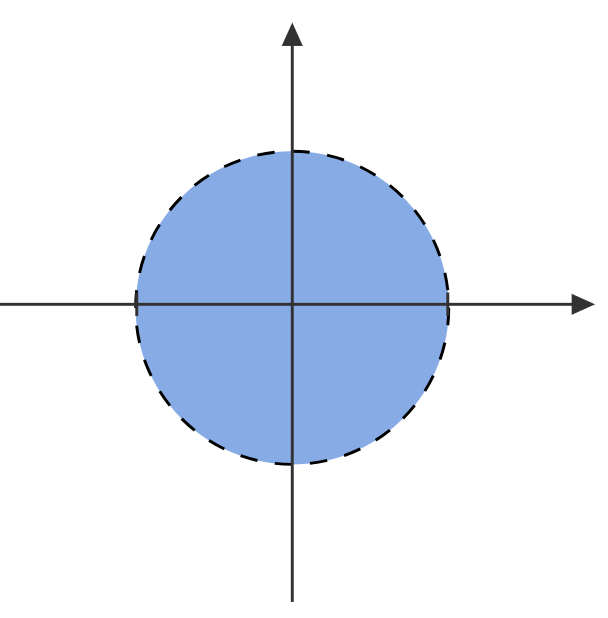
\includegraphics[width=.30\textwidth]{fig191}} \quad
    \subfloat[][\emph{Ball in }$\left( \RR^n, d_1\right)$]
    {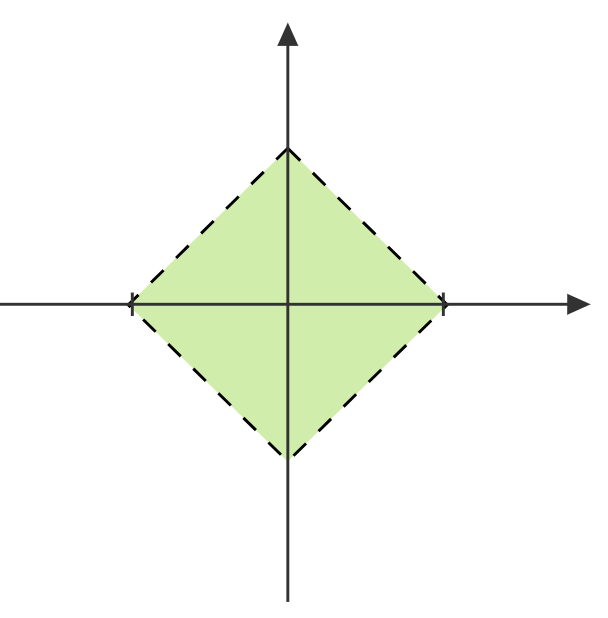
\includegraphics[width=.30\textwidth]{fig192}} \quad
    \subfloat[][\emph{Ball in }$\left( \RR^n, d_\infty\right)$]
    {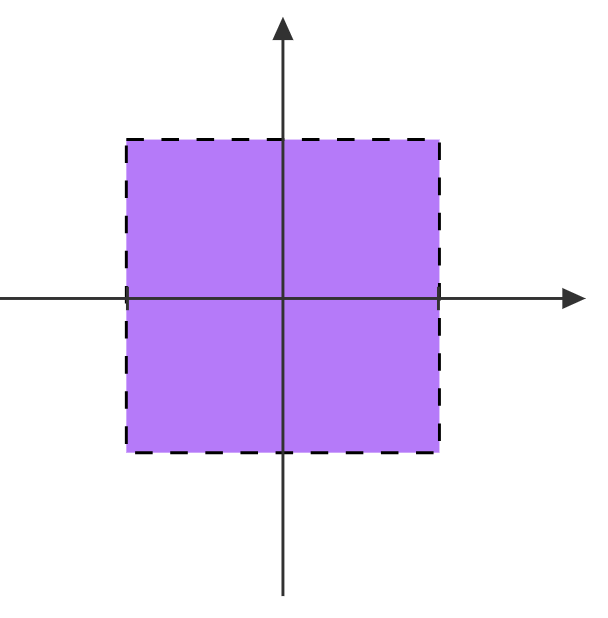
\includegraphics[width=.30\textwidth]{fig193}}
    %\caption*{Funzionamento del quicksort}
    %\label{fig:subfig}
\end{figure}
\end{enumerate}

It is remarkable that these balls are equivalent (we will explain it better in due time). 
\fg{0.4}{fig194}

\newpage

If you generalize to every $p$, you could say that
\fg{0.6}{fig195}

Furthermore, with $(X,d)$ where $d$ is the discrete metric, we have
\begin{equation*}
B_d(x_0,r)=\begin{cases}
    \gr{x_0}, &\text{ if }r\leq 1 \\
    X,&\text{ if }r>1    
\end{cases}
\end{equation*}

Therefore, many possible distances can be introduced on a set. In some cases they lead to the same \emph{structure} but not in genersal. For example, on $X=\Cc^0\left( [a,b] \right)$, $f,g\in X$, we have:
\begin{itemize}
    \item discrete distance (we've got it folks)
    \item $\displaystyle d_1(f,g):=\int_a^b\left| f(x)-g(x) \right|\dx$
    \item $\displaystyle d_\infty(f,g):=\max_{x\in[a,b]}\left| f(x)-g(x) \right|$
\end{itemize}

They are both distances on $\Cc^0\left( [a,b] \right)$ but they lead to different structures:
\fg{0.8}{fig196}

% section recall_on_metric_spaces (end)

\newpage

\section{Topology in metric spaces} % (fold)
\label{sec:topology_in_metric_spaces}

\begin{defn}
Let $(X,d)$ be a metric space and let $A\subset X$. For $x_0\in X$, we say that $x_0$ is:
\begin{enumerate}[(i)]
    \item an \textbf{interior point} of $A$ if
    \begin{equation*}
    \exists r>0\quad\text{s.t.}\quad B(x_0,r)\subset A
    \end{equation*}

    \item an \textbf{exterior point} of $A$ if
    \begin{equation*}
    \exists r>0\quad\text{s.t.}\quad B(x_0,r)\subset A^c:=X\setminus A
    \end{equation*}

    \item a \textbf{boundary point} of $A$ if it is neither interior nor exterior, i.e.
    \begin{equation*}
    B(x_0,r)\cap A\neq\varnothing\quad\text{and}\quad B(x_0,r)\cap A^c\neq\varnothing\quad\forall r>0
    \end{equation*}

    \item an \textbf{adherence point} of $A$ if it is either interior or boundary, i.e.
    \begin{equation*}
    B(x_0,r)\cap A\neq\varnothing\quad\forall r>0
    \end{equation*}

    \item an \textbf{accumulation point} of $A$ if
    \begin{equation*}
    \left( B(x_0,r)\cap A \right)\setminus \gr{x_0}\neq 0
    \end{equation*}

    \item an \textbf{isolated point} of $A$ if
    \begin{equation*}
    x_0\in A\quad\text{and}\quad \exists r>0\quad\text{s.t.}\quad B(x_0,r)\cap A=\gr{x_0}
    \end{equation*}

    \begin{marker}
    By definition, an isolated point cannot be an accumulation point.
    \end{marker}
\end{enumerate}

We also define:
\begin{equation*}
\left.
{\renewcommand*{\arraystretch}{1.5}
\begin{array}{ll}
\overset{o}{A}:=\left\{ x_o\in X\,:\, x_0\text{ is an interior point of }A \right\} &\textbf{interior}\text{ of }A \\
ext(A):=\left\{ x_o\in X\,:\, x_0\text{ is an exterior point of }A \right\} &\textbf{exterior}\text{ of }A \\
\partial A:=\left\{ x_o\in X\,:\, x_0\text{ is a boundary point of }A \right\} &\textbf{boundary}\text{ of }A \\
\overline{A}:=\left\{ x_o\in X\,:\, x_0\text{ is an adherence point of }A \right\} &\textbf{closure}\text{ of }A
\end{array}}
\right.
\end{equation*}
\begin{marker}
The definitions (i)-(ii)-(iii) are mutual disjoint, thus $\overset{o}{A},ext(A),\partial A$ are pairwise disjoint sets (see the property below).
\end{marker}
\end{defn}

\begin{defn}
A set $A\subset X$  is \textbf{open} if $A=\overset{o}{A}$. Similarly, $A$ is \textbf{closed} if $A^c$ is open.
\end{defn}

Let's take a look at some basic properties:
\begin{itemize}
    \item $\overset{o}{A},ext(A),\partial A$ form a partition of $X$
    \item $A$ open iff $A\cap\partial A=\varnothing$
    \item $\overline{A}=\overset{o}{A}\cup\partial A = A\cup\partial A$
    \item $A$ closed iff $A\equiv \overline{A}$
    \item $\overset{o}{A}$ is the largest (w.r.t. the inclusion order) open subset of $A$
    \item $\overline{A}$ is the smallest closed subset of $X$ containing $A$
    \item Let $I$ be a family of indexes (may be uncountable) and $A_i$ be an open set $\forall i\in I$. Then $\displaystyle\bigcup_{i\in I} A_i$ is open.
    \item Let $A_1,...,A_m$ for $m\in\NN$ be a finite number of open sets. Then $\displaystyle\bigcap_{i=1}^m A_i$ is open.
    \begin{home}
    Prove these last two properties.
    \end{home}
    \item Let $I$ be a family of indexes (may be uncountable) and $C_i$ be closed $\forall i\in I$. Then $\displaystyle\bigcap_{i\in I} C_i$ is closed.
    \item Let $C_1,...,C_m$ for $m\in\NN$ be closed. Then $\displaystyle\bigcup_{i=1}^m A_i$ is closed.
    \begin{subtle}
    These last two properties are deduced from the Morgan's laws.
    \end{subtle}
\end{itemize}

% section topology_in_metric_spaces (end)

\section{Limits for sequences} % (fold)
\label{sec:limits_for_sequences}

Let $(X,d)$ metric space, $\left\{ x_n \right\}_{n\in\NN}\subset X$ sequence, $x^*\in X$ point.

\begin{defn}
We say that $x_n\overset{d}\longrightarrow x^*$ as $n\to+\infty$ if
\begin{equation*}
\underbracket[0.2pt]{d(x_n,x^*)\to0}_{\text{limit in real numbers}}\text{ as }n\to+\infty
\end{equation*}
i.e.
\begin{equation*}
\forall\Ec>0\quad\exists \overline{n}=\overline{n}(\Ec)\in\NN\quad\text{s.t.}\quad \underbracket[0.2pt]{d(x_n,x^*)<\Ec}_{\text{or }x_n\in B_d(x^*,\Ec)}\quad \forall n>\overline{n}
\end{equation*}
\end{defn}

\begin{prp}
The limit (it it exists) is unique \underline{in metric space}.
\end{prp}

\begin{home}
Prove it.

\underline{Hint}: assuming by contraddiction that exist $x^*,y^*,x^*\neqy^*$ and then verify the triangular inequality.
\newline
\newline
\newline
\newline
\end{home}

\begin{prp}
If $\left\{ x_n \right\}_{n}$ converges to $x^*$, then any subsequence of $\left\{ x_n \right\}_{n}$ converges and it converges to $x^*$.
\end{prp}

\begin{defn}
A set $A\subset X$ is \textbf{sequentially closed} if for any converging sequence $\left\{ x_n \right\}_{n}\subset A$ its limit $x^*$ belongs to $A$.
\end{defn}

\begin{prp}
$A\subset X$ closed iff $A$ is sequentially closed.
\end{prp}

\begin{home}
Prove it.

\underline{Hint}: for ($\Rightarrow$) use the def. of closed, for ($\Leftarrow$) prove that $A=\overline{A}$ (i.e. $A\subset\overline{A}$ and $\overline{A}\subset A$).
\newline
\newline
\newline
\newline
\end{home}

% section limits_for_sequences (end)

\newpage

\section{Closure, Boundedness, Compactness} % (fold)
\label{sec:closure_boundedness_compactness}

% section closure_boundedness_compactness (end)

\section{Continuous functions in metric spaces} % (fold)
\label{sec:continuous_functions_in_metric_spaces}

% section continuous_functions_in_metric_spaces (end)

% chapter exercise_session_18_09 (end)